\documentclass[11pt,a4paper]{article}

% ---------------------------------------------------------------------------
% Reliable predictions from small cell populations: preparation dependence,
% measurement and certified count bounds.
%
% Author metadata: set the macros below before submission.  Author and
% affiliation are deliberately blank in this version.
% ---------------------------------------------------------------------------
\newcommand{\PaperAuthor}{}
\newcommand{\PaperAffiliation}{}
\newcommand{\PaperDate}{17 September 2026}

\usepackage[T1]{fontenc}
\usepackage[utf8]{inputenc}
\usepackage{lmodern}
\usepackage{microtype}
\usepackage[a4paper,margin=1.05in]{geometry}
\usepackage{amsmath,amssymb,amsthm,mathtools}
\usepackage{booktabs}
\usepackage{array}
\newcolumntype{L}[1]{>{\raggedright\arraybackslash}p{#1}}
\usepackage{enumitem}
\usepackage{graphicx}
\usepackage{xcolor}
\usepackage{capt-of}
\usepackage{placeins}
\usepackage[obeyspaces,spaces]{url}
\usepackage[numbers,sort&compress]{natbib}
\usepackage[colorlinks=true,linkcolor=blue!55!black,citecolor=blue!55!black,urlcolor=blue!55!black]{hyperref}
\hypersetup{pdftitle={Reliable predictions from small cell populations: preparation dependence, measurement and certified count bounds},
  pdfkeywords={branching processes, prediction intervals, low-cell-count assays, founder preparation, detection efficiency, stochastic domination, Lean}}

\DeclareUrlCommand\lean{\urlstyle{tt}}
\newcommand{\calibrationrows}{%
1024 & $\{N\leq 2\}$ & $C_n\leq 607$ & 0.01833462 & 0.02336813 & $19/20$ \\
1280 & $\{N\leq 2\}$ & $C_n\leq 759$ & 0.00994686 & 0.01284612 & $245/256$ \\
4000 & $\{N\leq 2\}$ & $C_n\leq 2374$ & 0.00002262 & 0.00003456 & $245/256$ \\
576 & $\{3,4\}$ & $H_n\geq 149$ & 0.01280508 & 0.01905814 & $0.95594491$ \\
640 & $\{3,4\}$ & $H_n\geq 165$ & 0.01055929 & 0.01284164 & $245/256$ \\}

\setlist{itemsep=2pt,topsep=3pt}
\setlength{\emergencystretch}{1.5em}

\theoremstyle{plain}
\newtheorem{theorem}{Theorem}[section]
\newtheorem{proposition}[theorem]{Proposition}
\newtheorem{lemma}[theorem]{Lemma}
\newtheorem{corollary}[theorem]{Corollary}
\theoremstyle{definition}
\newtheorem{definition}[theorem]{Definition}
\newtheorem{contract}[theorem]{Contract}
\theoremstyle{remark}
\newtheorem{remark}[theorem]{Remark}
\newtheorem{example}[theorem]{Example}

\newcommand{\R}{\mathbb R}
\newcommand{\N}{\mathbb N}
\newcommand{\PP}{\mathbb P}
\newcommand{\EE}{\mathbb E}
\newcommand{\Var}{\operatorname{Var}}
\newcommand{\Corr}{\operatorname{Corr}}
\newcommand{\TV}{\operatorname{TV}}
\newcommand{\cL}{\mathcal L}
\newcommand{\dd}{\mathrm d}
\newcommand{\ind}{\mathbf 1}
\newcommand{\Bin}{\operatorname{Binomial}}

\title{Reliable predictions from small cell populations:\\ preparation dependence, measurement\\ and certified count bounds}
\author{\PaperAuthor\\[2pt] {\small\itshape \PaperAffiliation}}
\date{\PaperDate}

\begin{document}
\maketitle

\begin{abstract}
Prediction from small cell populations depends on how the population was prepared and how it is observed, not only on the dynamics of individual lineages. We study upper prediction regions $\{0,\dots,k\}$ for the cell count at a fixed horizon in two-type branching models with inherited states, and ask which observations and assumptions justify a given cutoff $k$. First, we construct two founder preparations, one drawing a growth class independently for each founder and one giving every founder in a well the same class, that have identical observation laws for every single-founder experiment yet different minimal $95\%$ two-founder cutoffs, six and seven. Ordered-endpoint error accounting yields finite-sample marginal coverage for a data-selected cutoff without independence between calibration and the future population; an exact binomial calculation attains coverage at least $245/256$ from $640$ independent calibration wells, and a continuous preparation family identifies $\rho=3/5$ as the dependence level at which the minimal cutoff changes. Second, independent cell detection can erase or reverse the signal of a low-count statistic at efficiency one half, while a bounded generating-function statistic separates the preparations for every positive efficiency; thinning-invariant moment identities identify an unknown constant efficiency together with the preparation, and a feasible-set rule with bounded statistics keeps the coverage guarantee when the efficiency is unresolved. Third, one-sided stochastic comparisons give uniform recorded-count bounds under demographic, founder and false-object uncertainty: recorded count at most four with probability at least $0.9503$ for all birth rates up to $0.105$ and all death rates at least $0.05$ per time unit at horizon seven, and at most five with probability at least $0.9567$ for arbitrary death and switching rates when births are at most $0.1$. Fourth, for a reference inherited-state rate class with per-type $\ell^1$ uncertainty, a finite successful-history certificate proves recorded count at most three with probability at least $0.955935$, with three the smallest endpoint valid over the class. We separate theorems checked in Lean~4 from conventional extensions and exact computations, and report a documented lineage-data analysis that does not establish biological coverage. The results give explicit conditions for trustworthy count predictions and for measurements that justify smaller prediction regions.
\end{abstract}

\section{Introduction}\label{sec:intro}

\subsection{Prediction before mechanism}
A low-founder proliferation assay places a small number of cells in a well, waits a fixed time $T$, and records a count. A prediction region for that count is a set $\{0,\dots,k\}$ together with a guarantee $\PP(N_T\le k)\ge 0.95$, where $N_T$ is the true terminal count and the probability is over the preparation, the dynamics and, when a rule is learned from data, the calibration data. Such a region is useful precisely when it does \emph{not} require the experimenter to identify every hidden state or transition rate: a smaller region signals unusual outgrowth, a valid region protects against false alarms.

This article is about the conditions under which such a region can be trusted when the preparation, the hidden cellular states and the detector may differ from the setting in which the model was fitted. The thread has four parts.
\begin{enumerate}[label=(\roman*)]
\item A model that reproduces the expected count, and even the expected birth and death fluxes, can assign the wrong probability to small and large counts when phenotypic states are inherited. This is the subject of a companion manuscript~\citep{companion2026}; we do not repeat it, but the present results start from the same observation that averages do not determine tails.
\item Even a correct single-founder count law need not transfer to a different founder preparation. We give two preparations with \emph{identical} observation laws for every single-founder experiment and different minimal $95\%$ two-founder cutoffs (Section~\ref{sec:ambiguity}). Increasing the number of founders does not remove the discrepancy.
\item The measurement that repairs this must address the dependence relevant to the decision. Exact binomial and generating-function calculations show which two-founder statistics identify the preparation, how many wells are sufficient for a stated coverage, what a common detection efficiency does to the signal, and how to proceed when the efficiency is unknown (Sections~\ref{sec:decision} and~\ref{sec:detector}).
\item Some upper-count guarantees can be proved without resolving the mechanism at all, by one-sided comparison with a scalar birth--death process or with a finite family of successful histories (Sections~\ref{sec:safety} and~\ref{sec:inherited}).
\end{enumerate}

\subsection{Contributions}
The main results are stated for two-type continuous-time branching processes with inherited type, and the constants are exact rationals unless marked as displays.
\begin{itemize}
\item \textbf{Exact preparation ambiguity} (Theorem~\ref{thm:ambiguity}). Preparations~I and~W have equal single-family observation laws and two-founder cumulative distribution functions $F_I(k)=1-(k+5)/(4\cdot2^k)$ and $F_W(k)=1-(k+1)/2^{k+1}$; their minimal $95\%$ cutoffs are six and seven. For $m$ founders the variances are $\tfrac54 m$ and $m+\tfrac14 m^2$, and the independent-preparation $95\%$ quantile has coverage tending to $1/2$ under~W (Proposition~\ref{prop:many}). A continuous family $P_\rho=(1-\rho)P_I+\rho P_W$ has minimal cutoff six exactly when $\rho\le3/5$ (Proposition~\ref{prop:rho}).
\item \textbf{Direction-aware calibration} (Lemma~\ref{lem:nested}, Theorem~\ref{thm:adaptive}, Proposition~\ref{prop:tv}). For any rule with values in $\{6,7\}$, coverage under~I is at least $245/256$ and under~W at least $31/32$ minus the probability of selecting six, with no assumption relating calibration and the future well. The count-$\le2$ rule with $4000$, $1280$ or $1024$ wells and the counts-$3$-or-$4$ rule with $640$ or $576$ wells give uniform coverage $245/256$ or $19/20$, with exact integer certificates. A confidence rule for the dependence parameter certifies $\rho\le3/5$ with uniform coverage (Proposition~\ref{prop:rhorule}).
\item \textbf{The detector is part of the measurement} (Propositions~\ref{prop:reversal}--\ref{prop:feasible}). Under independent thinning with efficiency $d$, the count-$\le2$ gap is $d^3(2d-1)/(1+d)^4$, zero at $d=1/2$; the statistic $z^Y$ has gap $u^2(1-u)^2/(4(1+u)^2)$ with $u=d(1-z)$, positive for all $d>0$. The pair (efficiency, preparation) is identified by the first two factorial moments; a bounded feasible-set rule retains the coverage guarantee with unknown $d$; complete erasure is an obstruction.
\item \textbf{Uniform safety without resolving switching} (Theorem~\ref{thm:ratebox}, Propositions~\ref{prop:onesided}--\ref{prop:purebirth}). A recorded count at most four has probability at least $0.952037$ over a demographic box at horizon seven with arbitrary switching, arbitrary deletion, multiple-founder mass at most $0.001$ and false-object probability at most $0.01$; the proof uses only upper birth and lower death bounds, and pathwise domination extends it to births at most $0.105$ (cutoff four, bound above $0.9503$) and to arbitrary deaths with births at most $0.1$ (cutoff five, bound above $0.9567$).
\item \textbf{Robust inherited-state prediction} (Theorem~\ref{thm:three}). Over a reference rate class with per-type $\ell^1$ radius $0.0005$ per day, founder resistant probability within $0.001$ of $5/24$, horizon $\log 2/0.10001$ days, and the same preparation and false-object budgets, the recorded count is at most three with probability at least $6470259728405606661/6768514267000000000=0.955935\ldots$, and three is the smallest endpoint valid over the class. Endpoint four admits a $1\%$ inference-failure allowance.
\end{itemize}
Each claim is labelled by its evidence level (Section~\ref{sec:verification}): ``Lean-checked'' means that the statement, at the stated scope, is a compiled theorem in the accompanying Lean~4 development; ``conventional'' means a written proof in this article, with exact rational arithmetic replayed by a script that regenerates every printed constant and figure.

\subsection{Relation to existing work}
\citet{browning2025} study the practical identifiability of phenotypic adaptation from low-cell-count experiments with a stochastic model and several observation designs, and document the difficulty of distinguishing heterogeneity from alternative phenotype structures; see also \citet{browning2020} for identifiability of stochastic models in systems biology and \citet{iyer2025} for the role of inheritable states in drug-persister correlations. Our question is narrower and complementary: can two \emph{exactly} equivalent single-founder observation laws imply different count cutoffs after a preparation change, and which additional observation supports the appropriate cutoff? The phenomena motivating inherited-state models, persistence and drug tolerance without genetic change, are documented in \citet{balaban2004,sharma2010,shaffer2017}; the classical Luria--Delbr\"uck argument that fluctuations reveal mechanism goes back to \citet{luria1943}.

The mathematical components are established: branching generating functions and the linear birth--death law~\citep{yule1925,kendall1948,harris1963,athreyaney1972,kimmelaxelrod2015}, Hoeffding's inequality~\citep{hoeffding1963}, exact binomial confidence limits~\citep{clopper1934}, stochastic domination by coupling~\citep{lindvall1992}, finite-state truncation of master equations~\citep{munsky2006}, and asymmetric error control in ordered decisions~\citep{lehmannromano2005}. Distribution-free prediction~\citep{vovk2005,angelopoulos2023} supplies marginal guarantees from exchangeable calibration data; hierarchical data need attention to the sampling unit~\citep{lee2023}. Those methods do not by themselves justify transfer between founder preparations or a latent-count bound under an unspecified detector, and conversely the model-specific theorems here are not distribution-free. Our contribution is the explicit source-to-decision combination, the exact examples, the improved calibration and detector results, the broad one-sided demographic envelopes, and the verification boundary; we do not claim a general identifiability theorem, an optimal test, or biological validation.

\subsection{Evidence conventions}
Two kinds of evidence appear. \emph{Lean-checked} theorems are compiled in Lean~4~\citep{demoura2021} against mathlib~\citep{mathlib2020} with warnings treated as errors, and are named in the text by their declaration; they concern the encoded source process and the stated hypotheses, not the biological adequacy of either. \emph{Conventional} results have complete written proofs here; exact rational inequalities in them are additionally replayed by the accompanying script. Decimal values are downward-rounded displays of exact rationals unless they are marked numerical. A file hash identifies bytes, not correctness.

\section{Source model, prediction targets and contracts}\label{sec:model}

\subsection{The branching source}
The latent state is $X_t=(S_t,R_t)\in\N^2$ with total count $N_t=S_t+R_t$. A cell of type $a\in\{S,R\}$ divides into two cells of its type at rate $b_a$, dies at rate $d_a$, and switches type at rate $q_a$; the six rates are finite and nonnegative, with units inverse to the time unit. Cells evolve independently conditional on their initial states and on a possibly shared environment. Division increases the count by one, death decreases it by one, switching leaves it unchanged. Births are dominated by a Yule process of rate $\max(b_S,b_R)$ per cell and the remaining event rates are bounded on bounded population sets, so the process is nonexplosive~\citep{norris1997}. The labels $S$ and $R$ are model types; nothing below requires a biological interpretation of them.

\subsection{Targets}
Let $N_T$ be the true terminal count and let the recorded count be $Y_T=D+A$ with $D\le N_T$ the number of genuine cells detected and $A\in\N$ the number of false objects. An exceedance of cutoff $k$ begins at $k+1$. For a fixed source law $P$ the \emph{minimal $95\%$ cutoff} is $k_{.95}(P)=\min\{k\in\N:P(N_T\le k)\ge19/20\}$. For a data-selected cutoff $K=K(C)$ from calibration data $C$, \emph{marginal coverage} means $\PP(N_T\le K)\ge19/20$ with the probability including $C$, and \emph{certification of the model-specific cutoff} means $\PP(K=k_{.95})\ge1-\beta$. Neither implies coverage conditional on the realized value of $K$; that is a separate statement (Section~\ref{sec:baselines}).

\subsection{Three contracts}
The theorems use three source contracts, which must not be interchanged.

\begin{contract}[Menu calibration]\label{con:menu}
Exactly two founders per well; the source is one of two specified preparations~I and~W; normalized horizon $T=\log2$ in units of the fast birth rate; calibration wells are independent with perfect terminal counts; the future well has the same source marginal but may depend on the calibration wells.
\end{contract}

\begin{contract}[Uniform demographic safety]\label{con:box}
Preparation is empty, single-founder or multiple-founder with multiple-founder probability at most $\gamma$; horizon seven time units; per-cell rates in a stated set; arbitrary finite switching; detection may delete genuine cells arbitrarily; false objects appear with probability at most $\eta$.
\end{contract}

\begin{contract}[Inherited-state rate class]\label{con:class}
A reference rate vector with per-type $\ell^1$ uncertainty radius $0.0005$ per day, founder resistant probability within $0.001$ of $5/24$, a possibly shared static environment, physical horizon $T_0=\log2/0.10001\approx6.93078$ days, the same preparation and false-object budgets as Contract~\ref{con:box}, and arbitrary deletion.
\end{contract}

The two-founder example is normalized: assigning fast birth rate one per day makes its horizon about $0.693$ days; assigning $0.1$ per day makes it about $6.93$ days. Neither choice establishes biological calibration, and ``horizon seven'' in Contract~\ref{con:box} means seven time units. The cutoffs three, four, six and seven proved below belong to different contracts and cannot be compared without stating the contract.

\section{Exact preparation ambiguity}\label{sec:ambiguity}

\subsection{Construction}
At the reference rates $(b_S,d_S,q_S;b_R,d_R,q_R)=(0,0,0;1,0,0)$ a \emph{slow} family stays at one cell and a \emph{fast} family is a Yule process of rate one per cell. Its count $Z$ at $T=\log2$ satisfies
\begin{equation}\label{eq:yule}
\PP(Z=j)=2^{-j}\quad(j\ge1),\qquad g_0(z)=z,\qquad g_1(z)=\frac{z}{2-z},
\end{equation}
where $g_0,g_1$ are the slow and fast terminal generating functions; indeed the forward equations $p_j'=(j-1)p_{j-1}-jp_j$ from one cell are solved by $p_j(t)=e^{-t}(1-e^{-t})^{j-1}$.

In preparation~I each founder independently receives the slow or fast class with probability $1/2$ each. In preparation~W one class is drawn for the well and given to every founder. Conditional on the classes, families evolve independently in both preparations. ``Shared class'' names a dependence in the preparation; it does not assert that a persistent environmental cause has been identified.

\begin{theorem}[Equal single-founder observations, unequal predictions]\label{thm:ambiguity}
For any measurable observation of a single family's chronological trajectory, preparations~I and~W have equal observation laws. For two founders the terminal count distribution functions are, for $k\ge2$,
\begin{equation}\label{eq:cdf}
F_I(k)=1-\frac{k+5}{4\cdot2^k},\qquad F_W(k)=1-\frac{k+1}{2^{k+1}},
\end{equation}
and the minimal $95\%$ cutoffs are $k_{.95}(P_I)=6$ and $k_{.95}(P_W)=7$.
\end{theorem}

\begin{proof}
Let $P_0,P_1$ be the conditional family laws on a common measurable family space and $M=(P_0+P_1)/2$. The two-family laws are
\[
P_I=M\otimes M,\qquad P_W=\tfrac12P_0\otimes P_0+\tfrac12P_1\otimes P_1 .
\]
Both first-family marginals equal $M$, so every measurable observation of a single family has the same law under~I and~W. This is an identity of laws, not merely of moments, and it applies to the full chronological state, event and waiting-time trace.

For two founders, the initial-class mixtures are
\[
I:\ \tfrac14(\text{slow},\text{slow})+\tfrac12(\text{slow},\text{fast})+\tfrac14(\text{fast},\text{fast}),\qquad W:\ \tfrac12(\text{slow},\text{slow})+\tfrac12(\text{fast},\text{fast}),
\]
so the terminal generating functions are
\begin{equation}\label{eq:pgf}
G_I(z)=\frac{(g_0(z)+g_1(z))^2}{4},\qquad G_W(z)=\frac{g_0(z)^2+g_1(z)^2}{2}.
\end{equation}
The all-slow count is two. The mixed count is $1+Z$, with $\PP(1+Z\le k)=1-2^{-(k-1)}$. The all-fast count $Z_1+Z_2$ has the negative binomial law $\PP(Z_1+Z_2=j)=(j-1)2^{-j}$ for $j\ge2$, and writing $j=k+i$,
\[
\sum_{j>k}(j-1)2^{-j}=2^{-k}\Bigl[(k-1)\sum_{i\ge1}2^{-i}+\sum_{i\ge1}i\,2^{-i}\Bigr]=(k+1)2^{-k}.
\]
Hence $F_I(k)=\tfrac14+\tfrac12(1-2^{-(k-1)})+\tfrac14(1-(k+1)2^{-k})=1-(k+5)/(4\cdot2^k)$ and $F_W(k)=\tfrac12+\tfrac12(1-(k+1)2^{-k})=1-(k+1)/2^{k+1}$. In particular
\[
F_I(5)=\tfrac{59}{64}<\tfrac{19}{20}\le F_I(6)=\tfrac{245}{256},\qquad F_W(6)=\tfrac{121}{128}<\tfrac{19}{20}\le F_W(7)=\tfrac{31}{32},
\]
and monotonicity of a distribution function excludes every smaller cutoff.
\end{proof}

\begin{table}[t]
\centering
\caption{Exact two-founder model probabilities $\PP(N_T\le k)$ at $T=\log2$. These are model calculations, not empirical observations.}\label{tab:cdf}
\begin{tabular}{@{}cllll@{}}
\toprule
Cutoff $k$ & \multicolumn{2}{l}{Independent classes (I): $F_I(k)$} & \multicolumn{2}{l}{Shared class (W): $F_W(k)$}\\
\midrule
2 & $9/16$ & $=0.5625$ & $5/8$ & $=0.625$\\
5 & $59/64$ & $=0.921875$ & $29/32$ & $=0.90625$\\
6 & $245/256$ & $=0.95703125$ & $121/128$ & $=0.9453125$\\
7 & $125/128$ & $=0.9765625$ & $31/32$ & $=0.96875$\\
\bottomrule
\end{tabular}
\end{table}

\begin{remark}[What is Lean-checked]\label{rem:leanamb}
The single-family identity is compiled for the implemented chronological trace as \lean{chronological_single_observation_equal}, and the four inequalities defining the two minimal cutoffs as \lean{chronological_minimal_endpoints}, both in \lean{YuleAmbiguity.lean}. The formal proof does not assume the generating functions as an oracle: pure-birth paths keep the slow count fixed and never decrease the fast count, so killing paths once the fast count exceeds seven loses no successful history for the required thresholds, and a finite backward equation with exponential-sum solutions is checked by integer coefficient identities (\lean{yule_finite_exact}, \lean{source_cdf_formula}). The general-$k$ formula~\eqref{eq:cdf} is conventional. A genealogical-tree sample space is not separately implemented; the abstract mixture identity applies to it whenever it is supplied.
\end{remark}

This is a \emph{preparation-transfer obstruction}: the single-founder laws agree, and the target uses two founders under different dependence rules. It is not a contradiction in which one law has two quantiles.

\subsection{More founders do not remove shared uncertainty}
\begin{proposition}\label{prop:many}
For $m$ founders both preparations have mean $3m/2$, while
\begin{equation}\label{eq:var}
\Var_I(N_m)=\tfrac54m,\qquad \Var_W(N_m)=m+\tfrac14m^2 .
\end{equation}
Let $q_m$ be the minimal $95\%$ cutoff of $N_m$ under~I. Then $q_m/m\to3/2$ and $P_W(N_m\le q_m)\to1/2$.
\end{proposition}

\begin{proof}
The one-founder mixture law $M$ has mean $\tfrac12\cdot1+\tfrac12\cdot2=\tfrac32$ and second moment $\tfrac12\cdot1+\tfrac12\cdot6=\tfrac72$, hence variance $\tfrac54$; under~I the $m$ families are independent, which gives the first formula. Under~W the count is $m$ with probability $\tfrac12$ and a sum of $m$ independent geometric$(\tfrac12)$ variables (mean $2m$, variance $2m$) with probability $\tfrac12$, so $\EE N_m^2=\tfrac12m^2+\tfrac12(2m+4m^2)$ and $\Var_W(N_m)=m+\tfrac14m^2$. Under~I the strong law gives $N_m/m\to\tfrac32$, so for every $\varepsilon>0$, $P_I(N_m\le(\tfrac32+\varepsilon)m)\to1$ and $P_I(N_m\le(\tfrac32-\varepsilon)m)\to0$; hence $q_m/m\to\tfrac32$. Under~W, the slow branch has $N_m=m\le q_m$ eventually, while the fast branch has $N_m/m\to2>\tfrac32$, so $P_W(N_m\le q_m)\to\tfrac12\cdot1+\tfrac12\cdot0$.
\end{proof}

The law of large numbers operates correctly within each conditional population; the shared draw remains. This is persistent shared-condition uncertainty, not a failure of a limit theorem, and it is not evidence about any patient outcome.

\subsection{A continuous dependence family}
\begin{proposition}\label{prop:rho}
For $0\le\rho\le1$ let $P_\rho=(1-\rho)P_I+\rho P_W$: with probability $\rho$ the well uses a shared class draw, otherwise independent draws. Every single-founder observation law is unchanged, the founders' fast-class indicators have correlation $\rho$, and
\begin{equation}\label{eq:rho}
F_\rho(6)=\frac{245-3\rho}{256},\qquad F_\rho(7)=\frac{250-2\rho}{256},\qquad P_\rho(N_T\in\{3,4\})=\frac{19-5\rho}{64}.
\end{equation}
The minimal $95\%$ cutoff of $P_\rho$ is six if $\rho\le3/5$ and seven if $\rho>3/5$; equivalently, it is six exactly when $P_\rho(N_T\in\{3,4\})\ge1/4$.
\end{proposition}

\begin{proof}
Linearity of the mixture gives~\eqref{eq:rho} from Table~\ref{tab:cdf} and from $P_I(\{3,4\})=19/64$, $P_W(\{3,4\})=7/32$ (Lemma~\ref{lem:mass} below). $F_\rho(6)\ge19/20$ holds exactly when $3\rho\le245-243.2$, that is $\rho\le3/5$; $F_\rho(5)=(1-\rho)\tfrac{59}{64}+\rho\tfrac{29}{32}<19/20$ for every $\rho$; and $F_\rho(7)\ge31/32>19/20$ for every $\rho$. Finally $(19-5\rho)/64\ge1/4$ is again $\rho\le3/5$. The single-founder marginal fast probability is $1/2$ in both components, and the joint indicator law is $(1-\rho)$ times the product law plus $\rho$ times the diagonal law, which gives correlation $\rho$.
\end{proof}

Figure~\ref{fig:cutoffs} shows the two distribution functions and the continuous family. The observation criterion $P_\rho(N_T\in\{3,4\})\ge1/4$ turns the binary ambiguity into a quantitative question: the measurement need only establish that dependence lies below the level that changes the decision, not identify a mechanism.

\begin{figure}[t]
\centering
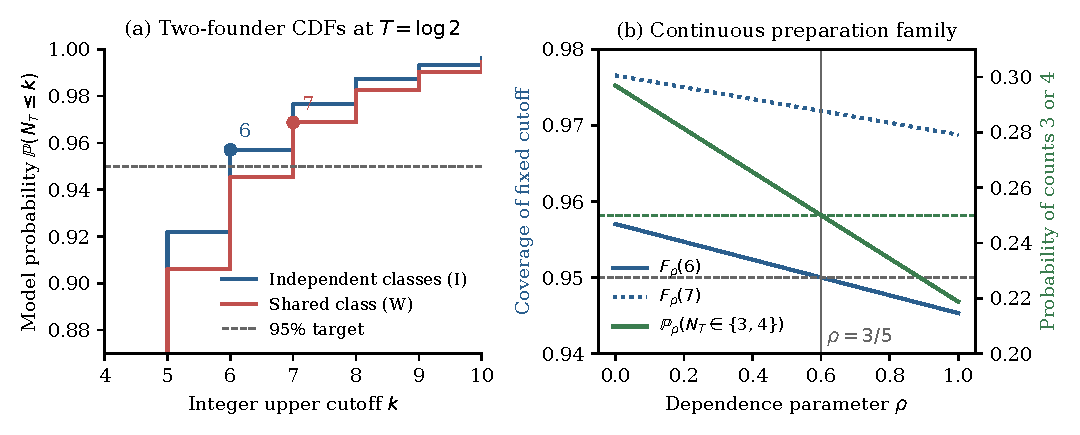
\includegraphics[width=\textwidth]{figures/cutoffs.pdf}
\caption{(a) Exact two-founder distribution functions of Theorem~\ref{thm:ambiguity}; the marked points are the minimal $95\%$ cutoffs six and seven. (b) The continuous family of Proposition~\ref{prop:rho}: the coverage of the fixed cutoff six crosses $19/20$ and the probability of counts three or four crosses $1/4$ at the same $\rho=3/5$. All values are model probabilities.}\label{fig:cutoffs}
\end{figure}

\section{Information for the decision}\label{sec:decision}

Throughout this section Contract~\ref{con:menu} holds. Let $N_1,\dots,N_n$ be the perfectly counted terminal counts of $n$ independent two-founder calibration wells, and let $N_T$ be the future two-founder count, with the same source marginal as the calibration wells but otherwise arbitrary dependence on them.

\subsection{Ordered-endpoint accounting}
\begin{lemma}[Nested endpoints]\label{lem:nested}
For any rule $K$ with values in $\{6,7\}$, measurable with respect to the calibration data, and any future count with the declared source marginal,
\begin{align}
P_I(N_T\le K)&\ge F_I(6)=245/256,\label{eq:nestI}\\
P_W(N_T\le K)&\ge\max\{F_W(6),\,F_W(7)-P_W(K=6)\}=\max\{121/128,\,31/32-e_W\},\label{eq:nestW}
\end{align}
where $e_W=P_W(K=6)$. More precisely, under either source, $\PP(N_T\le K)=F(7)-\PP(N_T=7,K=6)$.
\end{lemma}

\begin{proof}
Since $K\ge6$, $\{N_T\le6\}\subseteq\{N_T\le K\}$, giving both bounds at six. Since $\{N_T\le7\}=\{N_T\le K\}\cup\{N_T=7,K=6\}$ disjointly, $\PP(N_T\le K)=F(7)-\PP(N_T=7,K=6)\ge F(7)-\PP(K=6)$. Insert the source values from Table~\ref{tab:cdf}.
\end{proof}

No independence between calibration and the future count enters. An error under~I enlarges the region and cannot damage coverage; the dangerous decision is selecting six when~W is true. Given only $e_W$, the loss $\PP_W(N_T=7,K=6)$ is at most $\min\{e_W,P_W(N_T=7)\}=\min\{e_W,3/128\}$, and this extremal overlap is attainable over unrestricted couplings, so~\eqref{eq:nestW} is the best bound of its kind. Standard testing permits asymmetric error control~\citep{lehmannromano2005}; the point here is that the ordering of the endpoints makes one error harmless for coverage. The inclusions are compiled as \lean{nested_endpoint_lower} and \lean{upper_endpoint_loss} in \lean{Postproof.lean}.

\subsection{The low-count rule}
Let $X_i=\ind\{N_i\le2\}$ and $C_n=\sum_iX_i$. Theorem~\ref{thm:ambiguity} gives success probabilities $p_I=9/16$ and $p_W=5/8$, with midpoint $19/32$. Define
\begin{equation}\label{eq:oldrule}
K_n=\begin{cases}6,&C_n/n<19/32,\\7,&C_n/n\ge19/32.\end{cases}
\end{equation}

\begin{theorem}[Adaptive coverage]\label{thm:adaptive}
Rule~\eqref{eq:oldrule} has uniform marginal coverage at least $245/256=0.95703125$ under both preparations in each of the following cases: (i) $n=4000$, with the concentration proof compiled in Lean; (ii) $n=1280$, with the exact binomial certificate below. At $n=1024$ the same argument gives uniform coverage at least $19/20$. The future count need not be independent of calibration.
\end{theorem}

\begin{proof}
(i) The threshold is $1/32$ from either mean. Hoeffding's one-sided inequality for independent $[0,1]$ variables~\citep{hoeffding1963} gives $e_W,e_I\le\exp(-2n/32^2)=\exp(-125/16)\le1/2000$, the last step because the Taylor polynomial of degree $20$ of $\exp(125/16)$ already exceeds $2000$. Then $\min\{245/256,31/32-1/2000\}=245/256$ and Lemma~\ref{lem:nested} applies. This is compiled as \lean{adaptive_prediction_sharp}, which imports the source-connected concentration theorem \lean{classification_error}.

(ii) By independence and the Bernoulli means, $C_n\sim\Bin(n,p)$ under either source: each subset of $j$ successful wells has probability $p^j(1-p)^{n-j}$ and the $\binom nj$ such events partition $\{C_n=j\}$. Hence
\begin{equation}\label{eq:eWbinom}
e_W(n)=P_W\bigl(C_n\le\lceil19n/32\rceil-1\bigr)=8^{-n}\sum_{j=0}^{\lceil19n/32\rceil-1}\binom nj5^j3^{n-j}.
\end{equation}
The integer inequalities of Appendix~\ref{app:binomial} give $e_W(1024)\le3/160$ and $e_W(1280)\le3/256$. Since $31/32-3/160=19/20$ and $31/32-3/256=245/256$, Lemma~\ref{lem:nested} completes the proof.
\end{proof}

The first three rows of Table~\ref{tab:calibration} show the exact errors. These are sufficient sample sizes for this rule and this menu, not minimal ones, and adjacent sizes can behave nonmonotonically because the integer threshold jumps. The $1280$-well rule does not have $99.95\%$ label accuracy: its two errors are about $1.0\%$ and $1.3\%$. The conservative $4000$-well concentration bound supplies the stronger label guarantee. Coverage and label accuracy are different targets.

\subsection{A better separating event}
\begin{lemma}\label{lem:mass}
For $j\ge3$ the two-founder mass functions are $p_I(j)=(j+3)/2^{j+2}$ and $p_W(j)=(j-1)/2^{j+1}$, so $p_I(j)-p_W(j)=(5-j)/(4\cdot2^j)$; also $p_I(2)=9/16$, $p_W(2)=5/8$. Consequently the event $\{3,4\}$ attains the total variation distance:
\begin{equation}\label{eq:tv}
P_I(N_T\in\{3,4\})=\frac{19}{64},\qquad P_W(N_T\in\{3,4\})=\frac{7}{32},\qquad \TV(P_I,P_W)=\frac{5}{64}.
\end{equation}
\end{lemma}
\begin{proof}
Difference~\eqref{eq:cdf} at $k$ and $k-1$. The mass differences are positive exactly at $j\in\{3,4\}$, negative at $j=2$, zero at $j=5$ and negative beyond, so $\{3,4\}$ is the set of positive differences and its probability gap is the total variation distance.
\end{proof}

The count-$\le2$ event has gap $1/16=4/64$; the event $\{3,4\}$ has the largest gap $5/64$ among all events. Define
\begin{equation}\label{eq:newrule}
H_n=\sum_{i=1}^n\ind\{N_i\in\{3,4\}\},\qquad K'_n=\begin{cases}6,&H_n\ge\lceil33n/128\rceil,\\7,&\text{otherwise},\end{cases}
\end{equation}
where $33/128$ is the midpoint of $7/32$ and $19/64$. The orientation is reversed relative to~\eqref{eq:oldrule}: a high frequency of wells with three or four cells supports~I.

\begin{proposition}[Halving the sufficient calibration size]\label{prop:tv}
Under Contract~\ref{con:menu}, rule~\eqref{eq:newrule} with $n=640$ independent calibration wells has uniform marginal coverage at least $245/256$, and with $n=576$ at least $19/20$, without independence between calibration and the future count.
\end{proposition}

\begin{proof}
Under~W, $H_n\sim\Bin(n,7/32)$ and $e_W=P_W(H_n\ge\lceil33n/128\rceil)$. With $B_{n,c}=\sum_{j\ge c}\binom nj7^j25^{n-j}$, Appendix~\ref{app:binomial} verifies the integer inequalities
\begin{equation}\label{eq:tvcert}
160\,B_{576,149}\le3\cdot32^{576},\qquad 256\,B_{640,165}\le3\cdot32^{640},
\end{equation}
that is $e_W(576)\le3/160$ and $e_W(640)\le3/256$; here $\lceil33\cdot576/128\rceil=149$ and $\lceil33\cdot640/128\rceil=165$. Lemma~\ref{lem:nested} gives the two bounds; the~I bound $245/256$ holds for every rule with values in $\{6,7\}$.
\end{proof}

\begin{table}[t]
\centering
\caption{Calibration errors of the two rules from exact binomial sums. Decimals are downward-rounded displays; the certificates are integer inequalities. $e_W$ is the probability of selecting six under~W, $e_I$ the probability of selecting seven under~I. The last column is the uniform coverage lower bound from Lemma~\ref{lem:nested}.}\label{tab:calibration}
\begin{tabular}{@{}rllrrl@{}}
\toprule
$n$ & Event & Selects six when & $e_W$ & $e_I$ & Uniform bound\\
\midrule
\calibrationrows
\bottomrule
\end{tabular}
\end{table}

The new rule halves the sufficient size of Theorem~\ref{thm:adaptive}(ii) at nearly the same~I error (Table~\ref{tab:calibration}, Figure~\ref{fig:calibration}). It requires the full counts rather than the bit $\ind\{N_i\le2\}$. The event and threshold are fixed analytically before any data are seen; selecting among several such rules on the calibration sample would invalidate an unadjusted certificate. The largest single-event gap does not make the repeated Bernoulli test optimal among all procedures using complete counts: the likelihood ratio is $p_I(2)/p_W(2)=9/10$ and $p_I(j)/p_W(j)=(j+3)/(2(j-1))$ for $j\ge3$, and a likelihood-ratio or sequential procedure could be more efficient, but it needs its own exact error calculation and stopping rule; no optimality claim is made. A worked input: among $640$ qualifying wells, $H=164$ selects seven and $H=165$ selects six.

\begin{figure}[t]
\centering
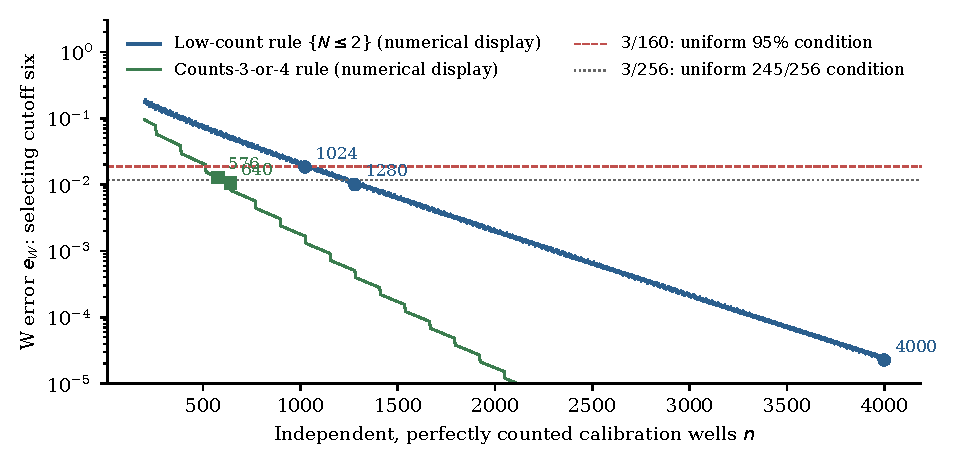
\includegraphics[width=0.9\textwidth]{figures/calibration.pdf}
\caption{The~W error controls the coverage guarantee. Curves are numerical renderings of the binomial tails for display; the marked sample sizes are the exact integer certificates of Table~\ref{tab:calibration}. The horizontal levels are sufficient conditions, not lower bounds on necessary sample size.}\label{fig:calibration}
\end{figure}

\subsection{What coverage alone does not identify}\label{sec:baselines}
Always returning seven is uniformly safe without calibration, since $F_I(7)=125/128$ and $F_W(7)=31/32$. Calibration therefore determines whether a smaller fixed cutoff is supported; it is not needed for the existence of a safe cutoff.

An independent external randomizer returning seven with probability $q$ and six otherwise has~W coverage $(1-q)\tfrac{121}{128}+q\tfrac{31}{32}$, which is at least $19/20$ exactly when $q\ge1/5$; at $q=1/5$ the mean endpoint is $6.2$, the~W coverage is exactly $19/20$ and the~I coverage is $123/128$. This rule learns nothing about the model. Its coverage conditional on returning six under~W is only $121/128$. A calibrated rule is therefore not claimed to be necessary or optimal for unconditional coverage with a small mean endpoint; its value is a data-based certification of the model-specific minimum with explicit error probabilities.

If the future count is additionally independent of calibration, conditioning on $K$ gives the exact coverages
\begin{equation}\label{eq:indep}
P_I(N_T\le K)=\frac{245}{256}+\frac{5e_I}{256},\qquad P_W(N_T\le K)=\frac{31}{32}-\frac{3e_W}{128}.
\end{equation}
The second expression exceeds $19/20$ as soon as $e_W\le4/5$. The large difference between this and the arbitrary-dependence requirement $e_W\le3/160$ explains why a sample-size statement must name its goal: robust coverage under arbitrary dependence, model-label recovery, or selection of the smallest justified endpoint. Thousands of wells are not necessary merely to obtain some $95\%$ marginal rule. Neither~\eqref{eq:nestW} nor~\eqref{eq:indep} implies coverage conditional on $K=6$, which under~W is $121/128$ whatever the calibration.

\subsection{Certifying a dependence tolerance}
\begin{proposition}\label{prop:rhorule}
Under Contract~\ref{con:menu} with the source $P_\rho$ of Proposition~\ref{prop:rho} for unknown $\rho\in[0,1]$, let $\theta=P_\rho(N_T\in\{3,4\})$ and let $L(C)$ be a lower confidence bound for a Bernoulli probability from $n$ independent trials with failure probability at most $\beta$ uniformly in the probability, for instance the exact Clopper--Pearson bound~\citep{clopper1934} applied to $H_n$. The rule ``six if $L(C)\ge1/4$, otherwise seven'' has marginal coverage at least $\min\{19/20,31/32-\beta\}$ for every $\rho$; in particular $\beta\le3/160$ gives uniform $95\%$ coverage over the whole family, without calibration--future independence.
\end{proposition}

\begin{proof}
If $\rho\le3/5$ then $F_\rho(6)\ge19/20$, so both endpoints cover by the inclusion $\{N_T\le6\}\subseteq\{N_T\le K\}$. If $\rho>3/5$ then $\theta<1/4$, so selecting six requires $L(C)\ge1/4>\theta$, an event of probability at most $\beta$; the identity in Lemma~\ref{lem:nested} then gives coverage at least $F_\rho(7)-\beta\ge31/32-\beta$.
\end{proof}

Seven is reported as a conservative fallback, not as proof that $\rho>3/5$. Near the boundary, strong confidence that six is justified requires substantial data; this is a real statistical boundary of the problem.

\section{The detector is part of the identifying measurement}\label{sec:detector}

This section changes the observation contract: conditional on the terminal population, each terminal cell is detected independently with the same probability $d\in[0,1]$, and there are no false objects. Then $Y\mid N\sim\Bin(N,d)$ and every generating function is evaluated at $w=1-d+dz$:
\begin{equation}\label{eq:thinpgf}
G^{(d)}_I(z)=\frac{(g_0(w)+g_1(w))^2}{4},\qquad G^{(d)}_W(z)=\frac{g_0(w)^2+g_1(w)^2}{2}.
\end{equation}

\subsection{Sign reversal and a bounded repair}
\begin{proposition}[The low-count signal vanishes at one half]\label{prop:reversal}
\begin{equation}\label{eq:reversal}
P_W(Y\le2)-P_I(Y\le2)=\frac{d^3(2d-1)}{(1+d)^4}.
\end{equation}
At $d=1/2$ the Bernoulli law of $\ind\{Y\le2\}$ is identical under~I and~W; for $d<1/2$ the ordering of the two means reverses.
\end{proposition}
\begin{proof}
Subtracting the two expressions in~\eqref{eq:thinpgf} gives $\tfrac14[g_0(w)-g_1(w)]^2=\tfrac14\bigl[w(1-w)/(2-w)\bigr]^2$. Thinning the fast law gives detected-count coefficients $(1-d)/(1+d)$ and $2d^i/(1+d)^{i+1}$ for $i\ge1$, and the slow law gives $1-d$ and $d$; convolving the appropriate mixtures and summing the coefficients of $z^0,z^1,z^2$ yields~\eqref{eq:reversal}. (The accompanying script performs this coefficient computation exactly at several rational $d$.)
\end{proof}

Even above one half the perfect-count midpoint cannot be reused, because both means have moved. The repair is to use a bounded statistic whose expectation is the generating function itself.

\begin{proposition}[Bounded repair]\label{prop:repair}
For known $d>0$ and fixed $0<z<1$, the statistic $z^Y\in[0,1]$ separates the preparations: with $u=d(1-z)\in(0,1)$,
\begin{equation}\label{eq:gap}
\Delta(d,z)=\EE_Wz^Y-\EE_Iz^Y=\frac{u^2(1-u)^2}{4(1+u)^2}>0 .
\end{equation}
For $n$ independent detected wells, classification by the midpoint of the two known expectations has each one-sided error at most $\exp(-n\Delta^2/2)$.
\end{proposition}
\begin{proof}
$\EE z^Y=G^{(d)}(z)$, so the gap is $\tfrac14[g_0(w)-g_1(w)]^2$ with $w=1-u$, which is~\eqref{eq:gap}. Each expectation is $\Delta/2$ from the midpoint; apply Hoeffding's inequality to the empirical mean of $[0,1]$-valued variables.
\end{proof}

At $z=d=1/2$ the two expectations are $729/1600$ and $369/800$, with gap $9/1600$: the vanished low-count signal does not mean equality of the complete observed laws. The repair is constructive but not sample-efficient: obtaining $e_W\le3/256$ from the Hoeffding bound at $d=z=1/2$ requires $n\ge2\ln(256/3)/\Delta^2$, that is $281{,}067$ wells. This is a sufficient size for this statistic and this concentration method, not a necessary one; strictly positive information is not the same as a practically efficient assay. Within the family~\eqref{eq:gap} the gap increases in $u$ up to $u^*=\sqrt2-1$ and decreases beyond, so for $d>u^*$ the choice $z=1-u^*/d$ maximizes it, and for $d\le u^*$ the supremum over $0<z<1$ is approached as $z\to0$, where $z^Y\to\ind\{Y=0\}$. This optimizes the expectation gap, not the error exponent or the experimental cost. Figure~\ref{fig:detection}(a) shows both gaps.

\begin{figure}[t]
\centering
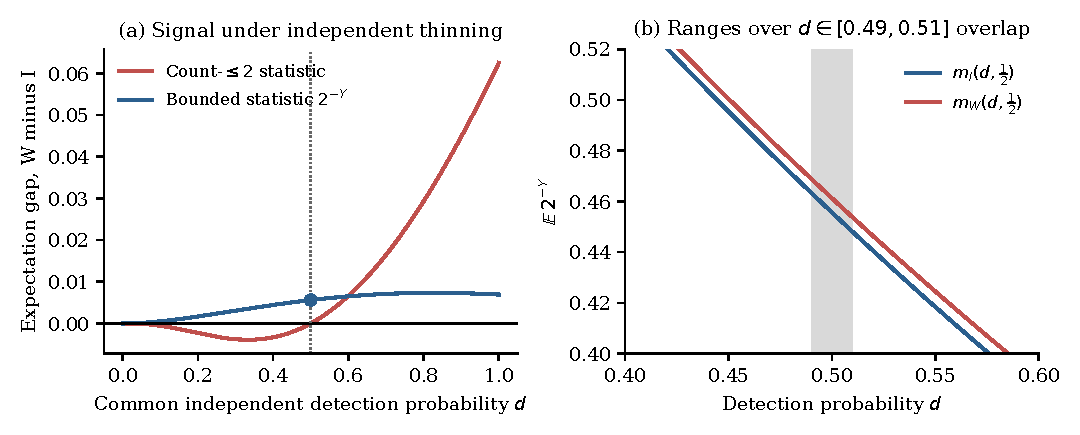
\includegraphics[width=\textwidth]{figures/detection.pdf}
\caption{(a) Exact expectation gaps under independent thinning: the count-$\le2$ statistic loses its signal at $d=1/2$ and reverses sign below, while the bounded statistic $2^{-Y}$ separates for every $d>0$; both gaps vanish at complete erasure. (b) The two generating-function expectations at $z=1/2$ as functions of $d$: over an efficiency interval $[0.49,0.51]$ their ranges overlap, so a single midpoint threshold cannot be certified (Section~\ref{sec:unknownd}). No detector efficiency has been estimated in this figure.}\label{fig:detection}
\end{figure}

\subsection{Complete erasure}
At $d=0$ both recorded laws are the point mass at zero. Any function of that law returns the same answer for~I and~W and cannot return both latent minimal cutoffs. This obstruction is compiled as \lean{deleted_count_cannot_identify_latent_cutoff} in \lean{DetectionBoundary.lean}. Propositions~\ref{prop:reversal} and~\ref{prop:repair} are conventional; no general thinning-source theorem is claimed in Lean. Unknown false objects, cell-dependent detection or shared fluctuations in detection invalidate their assumptions.

\subsection{Unknown constant efficiency}\label{sec:unknownd}
The midpoint rule of Proposition~\ref{prop:repair} assumes known $d$. Uncertainty in $d$ does not, however, make the preparations unidentifiable within the fixed menu; three questions must be separated: identifiability from the complete law, a finite-data confidence procedure, and sample efficiency.

\begin{proposition}[Joint identification]\label{prop:ident}
Both latent preparations have $\EE N=3$, and $\EE_I[N(N-1)]=17/2$, $\EE_W[N(N-1)]=9$. Under common independent thinning $\EE Y=3d$, $\EE_I[Y(Y-1)]=\tfrac{17}2d^2$, $\EE_W[Y(Y-1)]=9d^2$. Hence for unknown constant $d>0$ the complete observed law identifies both $d$ and the preparation, and the thinning-invariant ratio
\begin{equation}\label{eq:ratio}
\frac{\EE[Y(Y-1)]}{(\EE Y)^2}=\begin{cases}17/18,&\text{I},\\1,&\text{W},\end{cases}
\end{equation}
equals $(17+\rho)/18$ under $P_\rho$, identifying $\rho$ and $d$ jointly in that family.
\end{proposition}
\begin{proof}
$\EE_I[N(N-1)]=\Var_I N+9-3$ with $\Var_IN=5/2$ from~\eqref{eq:var}, and similarly $\Var_WN=3$. Binomial thinning multiplies the $r$-th factorial moment by $d^r$. The mean identifies $d=\EE Y/3$; equal observed laws at $d_I$ and $d_W$ would force $d_I=d_W$ and then $\tfrac{17}2d^2=9d^2$, impossible for $d>0$. Linearity in $\rho$ gives the last claim.
\end{proof}

These are population identities; plugging sample moments into~\eqref{eq:ratio} gives neither an exact confidence interval nor an unbiased estimator, and the argument uses the exact latent scale $\EE N=3$, the fixed horizon and the known menu. If birth rates, founder number or latent scale are also unknown, mean-based detector identification no longer follows. A finite-data rule that keeps the coverage guarantee with unresolved $d$ is nevertheless available with bounded statistics.

\begin{proposition}[A safe feasible-set rule]\label{prop:feasible}
Fix $L\ge2$, $0<z<1$ and $\beta_1,\beta_2>0$. From $n$ independent recorded wells of one preparation at common unknown efficiency $d$ compute
\[
\bar T=\frac1n\sum_i\min(Y_i,L),\qquad \bar V=\frac1n\sum_iz^{Y_i},\qquad a=L\sqrt{\frac{\ln(2/\beta_1)}{2n}},\qquad e=\sqrt{\frac{\ln(2/\beta_2)}{2n}},
\]
and with $R_L=(L+2)/2^L$ the detector interval $\mathcal D(C)=\bigl[\tfrac{\bar T-a}3,\tfrac{\bar T+a+R_L}3\bigr]\cap[0,1]$. Writing $m_M(d,z)=G^{(d)}_M(z)$ for $M\in\{I,W\}$, retain model $M$ if some $d\in\mathcal D(C)$ satisfies $|m_M(d,z)-\bar V|\le e$. Choose six only when~I is retained and~W is excluded; otherwise choose seven. Then
\begin{equation}\label{eq:feasible}
P_I(N_T\le K)\ge\frac{245}{256},\qquad P_W(N_T\le K)\ge\frac{31}{32}-(\beta_1+\beta_2),
\end{equation}
so the rule is uniformly at least $95\%$ when $\beta_1+\beta_2\le3/160$ and at least $245/256$ when $\beta_1+\beta_2\le3/256$.
\end{proposition}
\begin{proof}
Realize the thinning so that $Y\le N$ pathwise. Then $0\le\EE Y-\EE\min(Y,L)=\EE(Y-L)_+\le\EE(N-L)_+$, and summing the tails of Lemma~\ref{lem:mass},
\begin{equation}\label{eq:remainder}
\EE_I(N-L)_+=\frac{L+6}{2^{L+1}}\le\EE_W(N-L)_+=\frac{L+2}{2^L}=R_L\qquad(L\ge2).
\end{equation}
Hoeffding's two-sided inequality bounds $|\bar T-\EE\min(Y,L)|\le a$ except with probability $\beta_1$ and $|\bar V-m_M(d,z)|\le e$ except with probability $\beta_2$. On the intersection, $3d=\EE Y\in[\bar T-a,\bar T+a+R_L]$, so $d\in\mathcal D(C)$, and the true model satisfies the retention test. The true pair is therefore excluded with probability at most $\beta_1+\beta_2$. Under~W, output six requires that exclusion; apply Lemma~\ref{lem:nested}. The two statistics may use the same observations, and no calibration--future independence is used.
\end{proof}

The retention test is a finite calculation: for fixed $z$ both $m_I(\cdot,z)$ and $m_W(\cdot,z)$ are continuous and decreasing in $d$, so a model is feasible exactly when its range over the endpoints of $\mathcal D(C)$ meets $[\bar V-e,\bar V+e]$; an empty detector interval is reported explicitly. The rule solves validity with an uncertain constant detector at a conservative price: it does not guarantee frequent selection of six at small $n$. At $L=10$ the truncation remainder is $12/1024$, and sampling error can dominate it.

\paragraph{Detector controls.} If an independent control experiment yields $d\in[d_-,d_+]$ with failure probability at most $\beta_D$, a midpoint test is usable when $G=m_W(d_+,z)-m_I(d_-,z)>0$; the endpoints follow because both means decrease in $d$. For $z=1/2$, $[0.499,0.501]$ gives $G\approx0.0040965>0$, while $[0.49,0.51]$ gives $G\approx-0.0096619$ and the single-threshold certificate fails (Figure~\ref{fig:detection}(b)). Since a random control interval makes $G$ random, an unconditional guarantee should predeclare a gap requirement $g^*$, use the midpoint test only when $G\ge g^*$ and otherwise return seven; with controls independent of the classification wells and a stable common $d$,
\begin{equation}\label{eq:control}
e_W\le\beta_D+\exp(-n(g^*)^2/2),
\end{equation}
and Lemma~\ref{lem:nested} applies to this deterministic budget. The conservative fallback can increase the~I label error but not harm coverage.

\paragraph{Remaining boundaries.} As $d\to0$ both recorded laws concentrate at zero: $\PP(Y>0)\le\EE Y=3d$, so the total variation distance between the two $n$-well data laws is at most $6nd$ by comparison with the all-zero law and subadditivity over products. No fixed $n$ achieves uniform label accuracy over all $d>0$ without a positive efficiency floor; pointwise identifiability and uniform distinguishability differ. If efficiency varies randomly between wells, even independently of $N$, ratio~\eqref{eq:ratio} acquires the factor $\EE[d^2]/(\EE d)^2$, and a factor $18/17$ makes the~I value equal the~W constant-efficiency value: the moment diagnostic is confounded, although this does not assert equality of the full observed laws. Type-dependent detection, shared detection failures, population-dependent detection and false objects require new observation models.

\section{Uniform safety without resolving switching}\label{sec:safety}

This section uses Contract~\ref{con:box}. The switching rates are arbitrary finite nonnegative numbers, so the theorems hold without identifying the memory mechanism. Deletion is arbitrary, which makes an upper-count event easier to satisfy but can destroy all information about outgrowth; coverage of the recorded count and informativeness of the detector are reported separately.

\subsection{The compiled rate-box theorem}
\begin{theorem}[Recorded-count safety]\label{thm:ratebox}
Let the per-cell rates satisfy
\begin{equation}\label{eq:box}
b_S,b_R\in[1/10,\,501/5000],\qquad d_S,d_R\in[1/20,\,501/10000],\qquad T=7,
\end{equation}
with arbitrary finite switching rates and an arbitrary initial type for a single founder. Let the preparation be empty, single-founder or multiple-founder with multiple-founder probability at most $\gamma$ and an arbitrary multiple-founder law; let $D\le N_7$ be the genuine detected count and $\PP(A>0)\le\eta$. Then
\begin{equation}\label{eq:ratebox}
\PP(D+A\le4)\ge\frac{963}{1000}(1-\gamma)-\eta .
\end{equation}
In particular $\gamma\le0.001$ and $\eta\le0.01$ give $\PP(D+A\le4)\ge0.952037$.
\end{theorem}

\begin{proof}
For a function $f$ of the total count $n=s+r$, the typed generator is
\begin{equation}\label{eq:gen}
\cL f(s,r)=B(s,r)[f(n+1)-f(n)]+D_0(s,r)[f(n-1)-f(n)],\quad B=b_Ss+b_Rr,\ D_0=d_Ss+d_Rr,
\end{equation}
with vanishing rates at zero; switching cancels because it leaves $n$ unchanged. If $f$ is decreasing, then $B\le\lambda n$ with $\lambda=501/5000$ and $D_0\ge\mu n$ with $\mu=1/20$ give
\begin{equation}\label{eq:gencomp}
\cL f(s,r)\ge\lambda n[f(n+1)-f(n)]+\mu n[f(n-1)-f(n)] .
\end{equation}
Retain the counts zero through five and send an exit above five to an absorbing cemetery state six with payoff zero; count five must be retained because histories can return from five to four. On the retained states use the scalar rates $\lambda n,\mu n$ and the payoff $h(n)=\ind\{n\le4\}$, $h(6)=0$. The total scalar rate is at most $5(\lambda+\mu)=0.751<1$, so uniformization at rate one gives a stochastic matrix $P=I+Q$. It preserves nonnegative decreasing functions that vanish at six: for adjacent live states the coefficients of successive differences are nonnegative because $1-\lambda n-\mu(n+1)\ge0$ for $0\le n\le4$, and the cemetery boundary is immediate. Hence the scalar backward solution $v(t)=e^{tQ}h$ is decreasing for every $t$.

Apply~\eqref{eq:gencomp} to $v(t,\cdot)$ on the finite stopped typed state space: $v$ is a subsolution of the typed backward equation with the same initial payoff, so positivity of the finite Markov semigroup bounds the typed success probability below by $v(t,n)$. Equivalently, uniformize at a common clock rate bounding the typed rates, which may depend on the finite switching rates, and induct over clock steps using the preserved class of decreasing scalar test functions. Restoring the discarded histories can only increase the success probability, and the stopped-clock correspondence and nonexplosion transfer the inequality to the original source. Appendix~\ref{app:scalar} verifies $v(7,1)\ge963/1000$ by an exact rational certificate. Thus every allowed single-founder law, including any initial-type mixture, has $\PP(N_7\le4)\ge963/1000$. With preparation weights $e,w,m$ for empty, single and multiple founders,
\[
\PP(N_7\le4)\ge e+w\,(0.963)\ge(1-m)(0.963)\ge(1-\gamma)(0.963),
\]
and finally $\{N_7\le4\}\subseteq\{D+A\le4\}\cup\{A>0\}$ gives~\eqref{eq:ratebox} by subadditivity, with no independence assumption on the detector.
\end{proof}

The theorem is compiled as \lean{observed_four} in \lean{RateBox.lean}, with the scalar comparison in \lean{SourceLower.lean} and the rational certificate as \lean{finite_scalar_certificate}. The compiled source bound is $0.963$; the certificate value is $0.96355\ldots$ and the full scalar law gives more (Section~\ref{sec:domination}), but those are not substituted for the formal bound. Table~\ref{tab:budgets} lists sufficient budgets. The theorem does not prove that four is a minimal latent or recorded cutoff over the box, and it is not a detector-quality guarantee. The budgets $\gamma$ and $\eta$ are asserted allowances, not measured preparation or instrument performance.

\begin{table}[t]
\centering
\caption{Sufficient operating budgets from~\eqref{eq:ratebox}. These are mathematical allowances, not measured errors.}\label{tab:budgets}
\begin{tabular}{@{}lll@{}}
\toprule
Condition & Sufficient requirement & Consequence\\
\midrule
General $95\%$ target & $0.963\gamma+\eta\le0.013$ & coverage $\ge0.95$\\
$\gamma=0.001$ & $\eta\le0.012037$ & coverage $\ge0.95$\\
$\eta=0.01$ & $\gamma\le1/321$ & coverage $\ge0.95$\\
Compiled reference budgets & $\gamma=0.001,\ \eta=0.01$ & coverage $\ge0.952037$\\
\bottomrule
\end{tabular}
\end{table}

\subsection{The printed box is narrower than the proof needs}
\begin{proposition}\label{prop:onesided}
The conclusion~\eqref{eq:ratebox} holds, with the same certificate, under the one-sided conditions
\begin{equation}\label{eq:onesided}
0\le b_S,b_R\le501/5000,\qquad 1/20\le d_S,d_R<\infty,
\end{equation}
with arbitrary finite switching, the same preparation and observation budgets and the same horizon.
\end{proposition}
\begin{proof}
The comparison~\eqref{eq:gencomp} uses only $B\le\lambda n$ and $D_0\ge\mu n$; the lower birth limit and the upper death limit in~\eqref{eq:box} are never used. Finite-state stopping permits a clock depending on the actual finite rates of each model, so no common upper bound on death or switching rates is needed, and the birth cap gives nonexplosion for each model. The scalar certificate is unchanged.
\end{proof}
The relative width $0.2\%$ of each interval in~\eqref{eq:box} is therefore not the tolerance of the safety argument: it admits slow or nondividing cells and arbitrarily large death rates. The compiled theorem assumes the smaller box; the extension is conventional and is not relabelled as Lean-checked.

\subsection{Full scalar domination}\label{sec:domination}
\begin{lemma}[Pathwise domination]\label{lem:coupling}
If every cell has birth rate at most $\lambda$ and death rate at least $\mu$, whatever its type and however it switches, then the total count $N_t$ can be coupled with a linear birth--death process $Z_t$ with per-cell rates $\lambda,\mu$ and the same initial count so that $N_t\le Z_t$ for all $t$.
\end{lemma}
\begin{proof}
Match each actual cell to a dominating cell. A matched dominating cell proposes births at rate $\lambda$; each proposal is accepted as an actual birth with probability $b_{\text{type}}/\lambda\le1$, and the two new cells are matched. A death clock of rate $\mu$ removes a matched pair together; the actual cell carries an additional death clock of rate $d_{\text{type}}-\mu\ge0$, after which its partner continues as an unmatched dominating cell. Unmatched dominating cells evolve with rates $\lambda,\mu$. Switching only changes the rates attached to the matched actual cell. Every actual cell then has its own birth and death intensities, $Z$ is a linear birth--death process, and matching gives $N_t\le Z_t$ pathwise. Zero rates are handled by omitting their clocks; finite actual rates and the linear birth bound give nonexplosion. This is the standard coupling construction~\citep{lindvall1992}.
\end{proof}

\begin{lemma}[Linear birth--death law]\label{lem:bd}
For one initial cell, $\lambda\ne\mu$, $E=e^{-(\lambda-\mu)T}$ and
\[
a=\frac{\mu(1-E)}{\lambda-\mu E},\qquad q=\frac{\lambda(1-E)}{\lambda-\mu E},
\]
one has $\PP(Z_T=0)=a$, $\PP(Z_T=j)=(1-a)(1-q)q^{j-1}$ for $j\ge1$, and
\begin{equation}\label{eq:bdcdf}
\PP(Z_T\le k)=F_{\lambda,\mu,T}(k)=1-(1-a)q^k .
\end{equation}
For $\mu=0$ this is the Yule law $1-(1-e^{-\lambda T})^k$. In the critical case $\lambda=\mu$, $\PP(Z_T>k)=(\lambda T)^k/(1+\lambda T)^{k+1}$.
\end{lemma}
This is Kendall's classical result~\citep{kendall1948,bailey1964}; the generating function $g$ solves $\partial_tg=\lambda g^2-(\lambda+\mu)g+\mu$ with $g(0,z)=z$. Appendix~\ref{app:bd} records the monotonicity in $E$ used below. Under Contract~\ref{con:box} the two lemmas give $\PP(N_T\le k)\ge F_{\lambda,\mu,T}(k)$ for every single-founder law, without the finite-state loss of Theorem~\ref{thm:ratebox}: at $\lambda=501/5000$, $\mu=1/20$, $T=7$ the scalar value is $F_{\lambda,\mu,7}(4)\approx0.96642437695$ and the recorded bound is about $0.95545795258$ (numerical evaluations of a proved expression, not replacements for the compiled $0.952037$).

\begin{proposition}[A larger birth cap with cutoff four]\label{prop:broad}
If $0\le b_S,b_R\le0.105$, $d_S,d_R\ge0.05$ are finite, switching is arbitrary and finite, $T=7$, $\gamma\le0.001$ and $\eta\le0.01$, then
\begin{equation}\label{eq:broad}
\PP(D+A\le4)>0.95034241414>0.95 .
\end{equation}
\end{proposition}
\begin{proof}
Set $\lambda=21/200$, $\mu=1/20$, $x=(\lambda-\mu)\cdot7=77/200$ and $E_-=\sum_{j=0}^7(-x)^j/j!$. The odd Taylor truncation is a lower bound, $E_-\le e^{-x}=E$, by the sign of the remainder. By Appendix~\ref{app:bd}, $F_{\lambda,\mu,7}(4)$ is increasing in $E$ whenever $4\lambda\ge5\mu$, which holds here, so
\[
F_-=1-\frac{\lambda-\mu}{\lambda-\mu E_-}\Bigl[\frac{\lambda(1-E_-)}{\lambda-\mu E_-}\Bigr]^4\le F_{\lambda,\mu,7}(4)
\]
is a rational lower bound on the scalar probability. Exact arithmetic gives $\tfrac{999}{1000}F_--\tfrac1{100}>0.95034241414$. Lemmas~\ref{lem:coupling} and~\ref{lem:bd} give $\PP(N_7\le4)\ge F_-$ for every single-founder law, and the preparation and observation accounting of Theorem~\ref{thm:ratebox} completes the proof.
\end{proof}

\begin{proposition}[One extra count removes the death floor]\label{prop:purebirth}
If $0\le b_S,b_R\le0.1$, all death and switching rates are arbitrary finite nonnegative numbers, $T=7$, $\gamma\le0.001$ and $\eta\le0.01$, then
\begin{equation}\label{eq:purebirth}
\PP(D+A\le5)>0.95670013878>0.95 .
\end{equation}
\end{proposition}
\begin{proof}
Lemma~\ref{lem:coupling} with $\mu=0$ dominates $N$ by a Yule process of rate $0.1$, whose distribution function is $1-(1-e^{-0.7})^k$ and increases with $e^{-0.7}$. The odd truncation $r=\sum_{j=0}^7(-0.7)^j/j!=1191801547/2400000000\le e^{-0.7}$ gives $\PP(N_7\le5)\ge1-(1-r)^5$, and exact arithmetic gives $\tfrac{999}{1000}[1-(1-r)^5]-\tfrac1{100}>0.95670013878$. Accounting is as before.
\end{proof}

With the same pure-birth route, cutoff four gives only $0.9248\ldots$, so the extra count is needed when nothing is assumed about deaths. Table~\ref{tab:envelope} and Figure~\ref{fig:envelope} summarize the operating conditions. None of the rows establishes that an assay satisfies its conditions, and no minimality claim is made for the new cutoffs. The result admits a concrete tradeoff: a wider count region removes an entire demographic lower bound.

\begin{table}[t]
\centering
\caption{Sufficient source conditions at $T=7$ under the founder budget $\gamma\le0.001$ and false-object budget $\eta\le0.01$.}\label{tab:envelope}
\small
\begin{tabular}{@{}L{0.32\textwidth}cl L{0.36\textwidth}@{}}
\toprule
Per-cell rate conditions & Cutoff & Lower bound & Evidence\\
\midrule
Box~\eqref{eq:box} & 4 & $0.952037$ & Lean-checked (\lean{observed_four})\\
Births $\le0.1002$, deaths $\ge0.05$ & 4 & $0.952037$ & Conventional, Prop.~\ref{prop:onesided}; same certificate\\
Births $\le0.105$, deaths $\ge0.05$ & 4 & $>0.95034241414$ & Conventional, Prop.~\ref{prop:broad}; rational certificate\\
Births $\le0.1$, deaths arbitrary & 5 & $>0.95670013878$ & Conventional, Prop.~\ref{prop:purebirth}; rational certificate\\
\bottomrule
\end{tabular}
\end{table}

\begin{figure}[t]
\centering
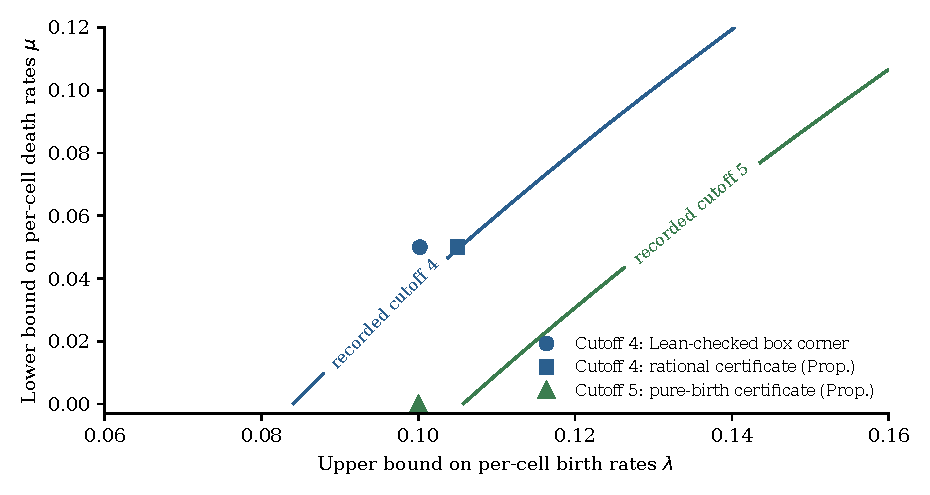
\includegraphics[width=0.85\textwidth]{figures/envelope.pdf}
\caption{Sufficient demographic conditions in the plane of birth cap $\lambda$ and death floor $\mu$. The curves are numerical level sets of $0.999\,F_{\lambda,\mu,7}(k)-0.01=0.95$ for recorded cutoffs $k=4$ and $k=5$ under full scalar domination (display only); the region above and to the left of a curve is sufficient for that cutoff. The three marked points are the proved operating points of Table~\ref{tab:envelope}. The Lean-checked corner lies strictly inside the cutoff-four region because the finite-state certificate discards histories that the full scalar law retains.}\label{fig:envelope}
\end{figure}

\section{Robust prediction under inherited-state rate uncertainty}\label{sec:inherited}

This section uses Contract~\ref{con:class}, in which the switching rates are small but uncertain and the founder type is random, so that a single-founder count law genuinely depends on the inherited state. Rates are per day.

\subsection{The class and the theorem}
The reference vector and the uncertainty set are
\begin{equation}\label{eq:class}
\begin{aligned}
a_0&=(b_S,d_S,q_S;\,b_R,d_R,q_R)=(0,\,0.3,\,0.001;\ 0.1,\,0,\,0.00001),\\
b_S+|d_S-0.3|+|q_S-0.001|&\le0.0005,\qquad |b_R-0.1|+d_R+|q_R-0.00001|\le0.0005,
\end{aligned}
\end{equation}
that is, two per-type $\ell^1$ balls of radius $0.0005$ intersected with the nonnegative orthant (not a six-coordinate rectangle). The horizon is $T_0=\log2/0.10001\approx6.93078$ days. Conditional on a single founder, its resistant probability satisfies $p\in[p_-,p_+]$ with $p_\pm=5/24\pm1/1000$. With a shared static environment $U$, these bounds hold for every conditional one-founder law, and the mixing law is the distribution of $U$ among single-founder preparations. Preparation and observation are as in Contract~\ref{con:box}: multiple-founder probability at most $\gamma$ with an arbitrary multiple-founder law, arbitrary deletion, and $\PP(A>0)\le\eta$.

\begin{theorem}[Robust endpoint three]\label{thm:three}
Under Contract~\ref{con:class}, put
\begin{equation}\label{eq:L3}
\begin{gathered}
a=\frac{599}{603},\qquad c=\frac{9950}{10051},\qquad r_3=\frac{1993}{4000}\Bigl(1+\frac c2+\frac{c^2}4\Bigr),\\
L_3=(1-p_+)a+p_+r_3=\frac{176701212731773153}{182749885209000000}.
\end{gathered}
\end{equation}
Then, also under conditional shared-environment mixing, $\PP(Y\le3)\ge\max\{0,(1-\gamma)L_3-\eta\}$. For $\gamma=1/1000$ and $\eta=1/100$,
\begin{equation}\label{eq:B3}
\PP(Y\le3)\ge B_3:=\frac{6470259728405606661}{6768514267000000000}=0.955935006291\ldots>\frac{19}{20}.
\end{equation}
At the reference rates with one founder, $p=5/24$ and perfect observation, every fixed endpoint below three has coverage strictly below $19/20$; thus three is the smallest fixed endpoint valid over the class.
\end{theorem}

The source theorem, its shared-environment extension, the accounting and the reference minimality are compiled as \lean{robust_endpoint_three_budget}, \lean{robust_endpoint_three_mixed_budget}, \lean{sharp_constant} and \lean{reference_minimum_endpoint} in \lean{LowFounderPrediction/}. The class is supplied, not estimated from the lineage data of Section~\ref{sec:empirical}. The theorem concerns a fixed time and endpoint, not a trajectory bound or an optional-stopping guarantee.

\subsection{Proof}
\paragraph{Finite successful histories.} The class~\eqref{eq:class} implies
\begin{equation}\label{eq:Q}
\begin{gathered}
b_S+d_S+q_S\le Q_S:=\tfrac{603}{2000},\qquad d_S\ge d_*:=\tfrac{599}{2000},\\
b_R+d_R+q_R\le Q_R:=\tfrac{10051}{100000},\qquad b_R\ge b_*:=\tfrac{199}{2000}.
\end{gathered}
\end{equation}
For $k\ge1$ retain the states $\mathcal K_k=\{0,S,R,2R,\dots,kR\}$ and send every exit to a cemetery $\partial$ with success value zero; every retained state has count at most $k$, and the killed chain follows the original until first exit, so its success probability is at most $\PP(N_t\le k)$ even when an omitted trajectory could later return. The physical-time comparison needs nonexplosion: with $V(s,r)=1+s+r$ the generator satisfies $\mathcal GV\le(b_S+b_R)V$, and stopping on finite sublevel sets, Gronwall's inequality and Markov's inequality show that infinitely many jumps in finite time have probability zero~\citep{norris1997}. The compiled chronological bridge transfers the killed comparison to the actual source measure.

\paragraph{Backward subsolution.} Set $E(t)=e^{-Q_Rt}$, $z(t)=c(1-E(t))$ with $c=b_*/Q_R$, and for $1\le n\le k$
\begin{equation}\label{eq:vn}
v_n(t)=\sum_{j=n}^k\binom{j-1}{n-1}E(t)^nc^{\,j-n}(1-E(t))^{j-n},\qquad v_{k+1}\equiv0 .
\end{equation}
These functions are nonnegative and, using $(j-n)\binom{j-1}{n-1}=n\binom{j-1}{n}$, satisfy $v_n'=nb_*v_{n+1}-nQ_Rv_n$ with $v_n(0)=1$. Put $v_0=1$, $v_S=a=d_*/Q_S$ and $v_\partial=0$. At $S$ the killed generator applied to $v$ is $d_Sv_0+q_Sv_1+b_S\cdot0-(b_S+d_S+q_S)a\ge d_*-Q_Sa=0=v_S'$, because the birth destination $SS$ is not retained and $v_1\ge0$. At $nR$ it is at least $nb_Rv_{n+1}-n(b_R+d_R+q_R)v_n\ge nb_*v_{n+1}-nQ_Rv_n=v_n'$, because retained death and switch destinations have nonnegative value and omitted destinations have value zero. At $0$ and $\partial$ both sides vanish. At time zero $v$ lies below the success indicator $h$ of the retained states. With $G$ the finite killed generator, whose exponential preserves coordinatewise nonnegativity, variation of constants gives
\[
e^{tG}h-v(t)=e^{tG}(h-v(0))+\int_0^te^{(t-u)G}\{Gv(u)-v'(u)\}\,\dd u\ge0 .
\]
Hence $\PP_S(N_t\le k)\ge a$ and $\PP_R(N_t\le k)\ge v_1(t)=E(t)\sum_{j=0}^{k-1}z(t)^j$. The $k=3$ subsolution and the source bridge are compiled; the argument for general $k$ is conventional.

\paragraph{Exact rationalization.} Since $T_0\le7$ (from $\log2\le7/10$) and $Q_R=0.10001+1/2000$,
\begin{equation}\label{eq:E}
E(T_0)=\tfrac12e^{-T_0/2000},\qquad \tfrac{1993}{4000}\le E(T_0)\le\tfrac12,\qquad 1-E(T_0)\ge\tfrac12,
\end{equation}
using $e^{-x}\ge1-x$; no numerical exponential enters. Substituting the lower bounds for $E$ and $z\ge c/2$ in $v_1$ gives the rational $r_3$ of~\eqref{eq:L3}. Since $r_3\le a$, the worst founder mixture over $p\in[p_-,p_+]$ is at $p_+$, and every conditional one-founder law has success probability at least $L_3$; integrating those laws over the environment preserves the bound without any independence between founder type and environment.

\paragraph{Accounting.} Empty preparations succeed with probability one. Discarding nonnegative multiple-founder contributions,
\begin{equation}\label{eq:prep}
\PP(N_{T_0}\le3)\ge e_0+wL_3=(1-m)L_3+e_0(1-L_3)\ge(1-\gamma)L_3,
\end{equation}
and $\{N_{T_0}\le3\}\cap\{A=0\}\subseteq\{D+A\le3\}$ gives $\PP(Y\le3)\ge\PP(N_{T_0}\le3)-\PP(A>0)$. Arbitrary dependence permits subtraction of $\eta$ but not multiplication by $1-\eta$: false objects concentrated on otherwise successful outcomes remove their entire mass. This proves~\eqref{eq:B3}.

\paragraph{Minimality.} At the reference source start with one resistant cell and retain only pure resistant birth histories without switching that end with $n\in\{3,\dots,7\}$ cells at $T_0$. With total per-cell event rate $b_R+q_R=0.10001$ and $e^{-(b_R+q_R)T_0}=1/2$ exactly, a history with $n-1$ events, all births, has probability $\tfrac12(c_0/2)^{n-1}$ with $c_0=b_R/(b_R+q_R)=10000/10001$. Each such history has $N_{T_0}\ge3$, so
\begin{equation}\label{eq:min}
\PP(N_{T_0}\ge3)\ge\frac5{48}\sum_{j=2}^6\Bigl(\frac{c_0}2\Bigr)^j>\frac1{20},
\end{equation}
by rational arithmetic; the complement shows that endpoint two, and every smaller endpoint, undercovers at an admissible source. This establishes uniform minimality over the class, not optimality of three for every individual source. \qed

\subsection{Endpoint four and a confidence allowance}
Applying the same proof with $k=4$ gives
\begin{equation}\label{eq:B4}
\begin{gathered}
r_4=\frac{1993}{4000}\sum_{j=0}^3\Bigl(\frac c2\Bigr)^j=\frac{941626977073717}{1015378162651000},\\
B_4=(1-\tfrac1{1000})L_4-\tfrac1{100}=\frac{16473049504746783406959}{17007584224404250000000}=0.968570802731\ldots,
\end{gathered}
\end{equation}
with $L_4=(1-p_+)a+p_+r_4$ and $r_4\le a$. This is a complete conventional proof; endpoint four is not source-connected in Lean. Suppose a confidence event $C$ has probability at least $1-\delta$ and that for almost every training data set in $C$ the \emph{conditional future} law satisfies the full contract with coverage at least $B$. Then $\PP(Y\le k)\ge\EE[\ind_C\PP(Y\le k\mid\text{training})]\ge(1-\delta)B$. With $\delta=0.01$,
\begin{equation}\label{eq:B4conf}
\tfrac{99}{100}B_4=0.958885094703\ldots>0.95,\qquad\text{whereas}\qquad \tfrac{99}{100}B_3<0.95 .
\end{equation}
This confidence multiplication requires the conditional-law premise; an estimated rate vector lying in a box does not establish it, and it is not the arbitrary-dependence menu theorem of Section~\ref{sec:decision}, which needs no such premise because the ordered endpoints make one error harmless. The accounting algebra is compiled as \lean{conditional_coverage_accounting}; the validity of a statistically estimated confidence region remains a separate obligation.

\begin{example}[All positive rates]
The rates $(0.0001,0.2999,0.0011;\,0.1001,0.0001,0.00002)$ per day have $\ell^1$ distances $0.0003$ and $0.00021$ from $a_0$, both within $0.0005$, so Theorem~\ref{thm:three} gives $B_3$ for them with arbitrary empty preparations. At $\eta=0.02$ the endpoint-three certificate falls below $0.95$; endpoint four restores the stated $1\%$ inference allowance at $\eta=0.01$. The zero-rate reference isolates the dependence mechanism; positive-rate examples show mathematical robustness but remain hypothetical operating points.
\end{example}

The short history family can be conservative when switching produces successful mixed-type descendants that are sent to the cemetery; increasing the endpoint alone cannot remove that loss, since the retained-history envelope has a ceiling in $k$. Successful-history loss, finite-state omission, observation budgets and statistical confidence losses are separate quantities and are kept separate above.

\section{Empirical scope and prospective use}\label{sec:empirical}

The mathematical examples are synthetic. A separate frozen comparison used recorded lineage families released with the lineage-tree hidden Markov study of \citet{mohammadi2022}; observed-phase count models were fitted to the annotations, not a reproduction of that study's model, and with a different target. One training run ($50$ families), one calibration run ($50$) and one test run ($75$) were used; predictions were frozen before test access; all families, including extinct ones, were retained. The target was the recorded descendant count of a family at a common frame. Rechecking the test workbook identified one absorbing extinction (a root dividing at frame $46$ with both daughters recorded dead at frame $54$), which corrects the outcome count to $51$ known and $24$ unresolved among $75$ without refitting or a new holdout.

\begin{table}[t]
\centering
\caption{Frozen, uncalibrated endpoints after the extinction correction: $51$ resolved and $24$ unresolved outcomes in one independent test run. Intervals are logical identification bounds on the realized fraction, not confidence intervals. Mean endpoint uses all $75$ predictions.}\label{tab:empirical}
\small
\begin{tabular}{@{}lccc@{}}
\toprule
Frozen model & Covered of $51$ known & Identification interval & Mean raw endpoint\\
\midrule
Exponential phases & $51$ & $[51/75,\,75/75]$ & $7.773$\\
Erlang-2 phases & $50$ & $[50/75,\,74/75]$ & $6.387$\\
Mean-composition scalar & $51$ & $[51/75,\,75/75]$ & $9.547$\\
Empirical training baseline & $49$ & $[49/75,\,73/75]$ & $6.000$\\
\bottomrule
\end{tabular}
\end{table}

If $c$ of $n-u$ resolved outcomes are covered and $u$ are unresolved, the realized coverage is identified only within $[c/n,(c+u)/n]$; both extremes are attainable. With $24/75>0.05$ unresolved, even all-success on the resolved set cannot bring the realized lower endpoint to $0.95$. These data establish neither biological $95\%$ coverage nor a comparative winner, and they neither refute the model nor the source study. Run-level calibration by the group-maximum rank rule of distribution-free prediction~\citep{vovk2005,angelopoulos2023,lee2023} returns an infinite endpoint with one calibration run, and nineteen calibration runs is merely the first potentially finite case for that rule. Constant predictors cannot retain an efficiency advantage after common residual calibration, since $a+(Y-a)_{(r)}=Y_{(r)}$; covariate-aware predictors can differ but still need independent evidence.

Prospective validation requires untouched independent runs, identical selection, a common horizon, explicit extinctions and censoring, founder records and detector controls. Fifty related families cannot replace fifty independent runs. Even for independent Bernoulli units with all successes, the one-sided exact $95\%$ lower confidence limit is $0.05^{1/n}$, so at least $59$ units are needed to exceed $0.95$. Table~\ref{tab:workflow} states, for each design step, what the results of this article resolve.

\begin{table}[t]
\centering
\caption{A design checklist derived from the theorems. Each row names the quantity a researcher records and the question it settles.}\label{tab:workflow}
\small
\begin{tabular}{@{}L{0.27\textwidth}L{0.68\textwidth}@{}}
\toprule
Step & What it resolves\\
\midrule
Define the event: true versus recorded count, horizon, endpoint, conditioning on preparation & Prevents a recorded-count guarantee being read as latent eradication (Section~\ref{sec:model}).\\
Define the sampling unit: well and shared batch or run; related cells grouped & Determines whether the independence premise of calibration is credible (Sections~\ref{sec:decision},~\ref{sec:empirical}).\\
Establish the preparation: founder count and its uncertainty, empty and multiple-founder frequencies & Determines which source law is predicted and the budget $\gamma$ (Sections~\ref{sec:ambiguity},~\ref{sec:safety}).\\
Specify observation: detection mechanism, constant versus variable efficiency, false objects & Selects the applicable theorem and statistic and the budget $\eta$ (Section~\ref{sec:detector}).\\
Obtain a baseline: fixed seven for the menu, or a scalar envelope for a justified demographic class & Supplies a conservative prediction before any smaller-cutoff calibration (Sections~\ref{sec:baselines},~\ref{sec:safety}).\\
Add a discriminating measurement: full two-founder counts, or the detector-aware statistics & Addresses the dependence that changes the cutoff (Propositions~\ref{prop:tv},~\ref{prop:rhorule},~\ref{prop:feasible}).\\
Compare decisions at matched guarantees: coverage, selection frequencies, endpoint size & Prevents a narrower uncalibrated region from being declared superior (Section~\ref{sec:baselines}).\\
Validate prospectively on untouched units with an ascertainable common endpoint & Tests whether the source and observation assumptions support actual use (Section~\ref{sec:empirical}).\\
\bottomrule
\end{tabular}
\end{table}

\section{Verification, reproducibility and limitations}\label{sec:verification}

\subsection{Evidence map}
Table~\ref{tab:evidence} lists every claim used above with its evidence level. The Lean development uses Lean~4 (toolchain \lean{v4.30.0}) with mathlib, compiled with warnings treated as errors and with transitive source dependencies materialized; the exported declarations were probed for their elaborated types. Kernel checking establishes consequences of the encoded source process and hypotheses. It does not establish biological adequacy of the model, the validity of an estimated rate region, or clinical utility. The Lean statements name measures on an implemented chronological jump-trajectory space and connect the finite killed comparisons to the actual source measure through a compiled bridge, so no premise assumes the desired distribution function.

\begin{table}[t]
\centering
\caption{Evidence level of each claim. Lean names are declarations in the accompanying development (directories \texttt{MemoryPrediction/} and \texttt{LowFounderPrediction/}); ``conventional'' means a written proof in this article with exact arithmetic replayed by the checking script.}\label{tab:evidence}
\small
\begin{tabular}{@{}L{0.36\textwidth}L{0.59\textwidth}@{}}
\toprule
Claim & Evidence\\
\midrule
Single-founder observation equality (Thm.~\ref{thm:ambiguity}) & Lean: \lean{chronological_single_observation_equal}; general family-space identity in \lean{SharedEnvironment.lean}. No genealogical-tree implementation.\\
Cutoffs six and seven (Thm.~\ref{thm:ambiguity}) & Lean: \lean{chronological_minimal_endpoints}, \lean{source_cdf_formula}; general-$k$ formula~\eqref{eq:cdf} conventional.\\
Many founders (Prop.~\ref{prop:many}); continuous family (Prop.~\ref{prop:rho}) & Conventional.\\
Nested endpoints (Lemma~\ref{lem:nested}) & Lean: \lean{nested_endpoint_lower}, \lean{upper_endpoint_loss}.\\
$4000$-well coverage $245/256$ (Thm.~\ref{thm:adaptive}(i)) & Lean: \lean{classification_error}, \lean{adaptive_prediction_sharp}.\\
$1280$- and $1024$-well coverage (Thm.~\ref{thm:adaptive}(ii)) & Conventional binomial law plus exact integer certificates (Appendix~\ref{app:binomial}).\\
$640$- and $576$-well rule (Prop.~\ref{prop:tv}); $\rho$ confidence rule (Prop.~\ref{prop:rhorule}) & Conventional; exact integer certificates~\eqref{eq:tvcert}.\\
Fixed and randomized baselines; independence formulas~\eqref{eq:indep} & Conventional algebra from exact source values.\\
Sign reversal and bounded repair (Props.~\ref{prop:reversal},~\ref{prop:repair}) & Conventional; exact rational examples.\\
Complete erasure & Lean: \lean{deleted_count_cannot_identify_latent_cutoff}.\\
Unknown-$d$ identification and feasible-set rule (Props.~\ref{prop:ident},~\ref{prop:feasible}) & Conventional.\\
Rate-box bound $0.952037$ (Thm.~\ref{thm:ratebox}) & Lean: \lean{observed_four}, \lean{source_scalar_lower}, \lean{finite_scalar_certificate}. No minimality claim.\\
One-sided conditions, broad caps, pure-birth (Props.~\ref{prop:onesided}--\ref{prop:purebirth}) & Conventional; rational certificates (Appendix~\ref{app:bd}).\\
Endpoint three, mixing, minimality (Thm.~\ref{thm:three}) & Lean: \lean{robust_endpoint_three_budget}, \lean{robust_endpoint_three_mixed_budget}, \lean{sharp_constant}, \lean{reference_minimum_endpoint}, \lean{preparation_budget}.\\
Endpoint four and confidence allowance~\eqref{eq:B4}--\eqref{eq:B4conf} & Conventional source proof; accounting algebra Lean: \lean{conditional_coverage_accounting}.\\
Empirical comparison (Section~\ref{sec:empirical}) & Frozen predictions and annotation audit; identification bounds only.\\
Biological applicability; clinical performance & Not established in this work.\\
\bottomrule
\end{tabular}
\end{table}

\subsection{Reproducibility}
The accompanying script \lean{check_paper.py} replays every exact constant in this article with rational and integer arithmetic (the distribution functions and mass functions from the convolution of single-founder laws, the binomial certificates by an exact integer recurrence, the sixteen-row scalar certificate, the odd Taylor lower bounds, the linear birth--death rational bounds, the class constants $L_3,B_3,r_4,B_4$ and the minimality witness), verifies that every printed decimal is a downward rounding of its exact value, checks the closed-form linear birth--death law against a numerical solution of the forward equations, and regenerates all four figures. It runs in well under a minute and exits nonzero on the first failed check. The manuscript build consumes only retained figures and generated table rows; it does not run a stochastic search or refit the empirical comparison.

\subsection{Limitations and claims to avoid}
The menu theorems fix the source to two preparations at a normalized horizon and assume independent, perfectly counted calibration wells; a recorded well identifier is not proof of independence, and wells on one plate may share batch effects. The demographic envelopes assume the stated one-sided rate bounds; no assay has been shown to satisfy them. The inherited-state class is supplied, not estimated. Constant common detection is a model; type-dependent, shared or population-dependent detection needs new observation models. No count exceedance in these models demonstrates genetic resistance, persister cells, treatment failure or patient risk, and no dosing or maintenance recommendation follows. A larger cutoff reduces false exceedances under a null model while reducing sensitivity to a genuine alternative; that tradeoff requires an alternative distribution and a decision or power analysis that this article does not supply. Optimal sample sizes, sequential procedures and general detector models are open and are not needed for the claims made here.

\FloatBarrier
\appendix

\section{Exact binomial certificates}\label{app:binomial}
For a Bernoulli probability $a/b$ define the integers $a_0=(b-a)^n$ and $a_{j+1}=a(n-j)a_j/((b-a)(j+1))$; induction gives $a_j=\binom nja^j(b-a)^{n-j}$, so every division is exact and $\sum_{j\le k}a_j/b^n$ is the binomial distribution function at $k$. The five certificates used in Section~\ref{sec:decision} are the following integer inequalities.
{\allowdisplaybreaks
\begin{gather*}
160\sum_{j\le607}\binom{1024}{j}5^j3^{1024-j}\le3\cdot8^{1024},\\
256\sum_{j\le759}\binom{1280}{j}5^j3^{1280-j}\le3\cdot8^{1280},\\
256\sum_{j\le2374}\binom{4000}{j}5^j3^{4000-j}\le3\cdot8^{4000},\\
160\sum_{j\ge149}\binom{576}{j}7^j25^{576-j}\le3\cdot32^{576},\\
256\sum_{j\ge165}\binom{640}{j}7^j25^{640-j}\le3\cdot32^{640}.
\end{gather*}}
The first row bounds $e_W$ for the low-count rule~\eqref{eq:oldrule} at $n=1024,1280,4000$; the second bounds $e_W$ for the counts-$3$-or-$4$ rule~\eqref{eq:newrule} at $n=576,640$. The thresholds are $\lceil19n/32\rceil-1=607,759,2374$ and $\lceil33n/128\rceil=149,165$. The script evaluates these with the recurrence above and no floating-point arithmetic; the~I errors in Table~\ref{tab:calibration} are computed the same way. These are exact computations supporting conventional theorems, not statements trusted by the Lean kernel; the compiled $4000$-well theorem uses the Hoeffding route instead.

\section{The finite scalar certificate}\label{app:scalar}
Let $Q$ be the seven-state generator of the scalar killed chain in Theorem~\ref{thm:ratebox} (live states $0,\dots,5$, cemetery six) and $P=I+Q$. Nonnegativity of the Poisson weights gives
\[
v(7,1)=e^{-7}\sum_{j\ge0}\frac{7^j}{j!}(P^jh)(1)\ge e^{-7}\sum_{j=0}^{15}\frac{7^j}{j!}(P^jh)(1).
\]
Set $M=10^6$, $a_{0,i}=M\ind\{i\le4\}$, $a_{j,6}=0$, and for $0\le i\le5$
\begin{equation}\label{eq:rows}
a_{j+1,i}=\Bigl\lfloor\frac{(5000-751i)a_{j,i}+501i\,a_{j,i+1}+250i\,a_{j,\max(i-1,0)}}{5000}\Bigr\rfloor .
\end{equation}
All coefficients are nonnegative, so induction gives $a_{j,i}/M\le(P^jh)(i)$. The sixteen values at the initial state are
\begin{center}\small
\begin{tabular}{@{}lrrrrrrrr@{}}
\toprule
$j$ & 0 & 1 & 2 & 3 & 4 & 5 & 6 & 7\\
$a_{j,1}$ & 1000000 & 1000000 & 1000000 & 1000000 & 997580 & 992141 & 983746 & 972743\\
\midrule
$j$ & 8 & 9 & 10 & 11 & 12 & 13 & 14 & 15\\
$a_{j,1}$ & 959583 & 944728 & 928611 & 911617 & 894077 & 876268 & 858418 & 840711\\
\bottomrule
\end{tabular}
\end{center}
Since $e<271829/100000$ and the seventh power of that rational is below $1097$, $e^{-7}\ge1/1097$, and exact rational arithmetic yields
\[
\frac1{1097\cdot10^6}\sum_{j=0}^{15}\frac{7^j}{j!}a_{j,1}=\frac{3134312565151423153}{3252877056000000000}=0.9635508847\ldots>\frac{963}{1000}.
\]
Only the rational lower bound $963/1000$ is used. Lean checks the initial rows, each step inequality, nonnegativity, the exponential bound and the final comparison (\lean{ScalarCertificate.lean}). The finite lower comparison is related to finite-state projection~\citep{munsky2006}, but the source-to-scalar inequality is proved separately here.

\section{The linear birth--death law and its monotonicity}\label{app:bd}
With $E=e^{-(\lambda-\mu)T}$, $\lambda\ne\mu$, the generating function of $Z_T$ from one cell is $g(z)=\bigl(a+(1-a-q)z\bigr)/(1-qz)$ with $a,q$ as in Lemma~\ref{lem:bd}; expanding in $z$ gives the stated masses and~\eqref{eq:bdcdf}. For $\mu\to0$, $a\to0$ and $q\to1-E$, the Yule law. Regard the tail $t(E)=(1-a)q^k$ as a function of $E\in(0,1)$ at fixed $\lambda,\mu$; for $k=4$,
\[
\frac{\dd}{\dd E}\log t(E)=\frac{5\mu-4\lambda-\mu E}{(1-E)(\lambda-\mu E)},
\]
a closed form the script verifies symbolically. The denominator is positive on $(0,1)$ because $\lambda>\mu E$, and the numerator is negative whenever $4\lambda\ge5\mu$. Hence $F_{\lambda,\mu,T}(4)$ increases with $E$, and any rational $E_-\le E$ gives a rational lower bound on $F$. In Proposition~\ref{prop:broad}, $E_-$ is the degree-seven Taylor polynomial of $e^{-x}$ at $x=77/200$, whose signed remainder makes it a lower bound. The same route at the corner $\lambda=501/5000$, $\mu=1/20$ of box~\eqref{eq:box} gives a recorded bound above $0.95545$, confirming that the finite-state certificate of Appendix~\ref{app:scalar} is conservative.

\paragraph{Preparation statement.} This manuscript and its accompanying artifacts were prepared with AI assistance. No collaborator authorship, institutional affiliation, external peer review or publication acceptance is asserted. Author and affiliation fields are intentionally blank in this version.

\bibliographystyle{plainnat}
\bibliography{references,extra_refs}

\end{document}
